% Chapter 4

\chapter{Method} % Main chapter title

\label{Method} % For referencing the chapter elsewhere, use \ref{Chapter1} 

\lhead{Chapter 4. \emph{Method}} % This is for the header on each page - perhaps a shortened title


In this chapter an introduction to the problem specifications and a comprehensive documentation describing the methods used is given. As an initial experiment, a random methodology to generate soft robot morphologies is implemented to verify that random non-evolutionary approaches fail in such settings. Next, evolutionary methods are used in order the morphology and the locomotion strategy of soft robots to be simultaneously evolved in the simulated environment. A direct encoded genome is used within a simple genetic algorithm as in~\citep{cheney2013unshackling}. This direct encoded GA is expected to be unable to evolve efficient locomotion due to the irregular morphologies direct encoding is producing. Furthermore, a generative encoding method is used and paired with the NEAT evolutionary algorithm in order to establish a baseline for the following experiments, verifying previous work~\citep{cheney2013unshackling}.

Pure novelty search was applied in the evolution of three-dimensional virtual creatures in a simulated environment~\citep{lehman2011evolving} using as a behavior metric the morphology of the produced creatures, where it failed to compete with the traditional fitness based search method. Novelty search is the main search methodology investigated in this thesis. The implementation of this method alters the pipeline of the NEAT and any evolutionary algorithm to fit the new objective function. In addition to the discussion regarding the algorithm of novelty search, different behavior metrics that can be used in this problem task are defined.



\section{Problem Introduction}
Recent work in evolutionary robotics shows that compositional pattern-producing networks (CPPNs) can encode soft robot morphologies. These networks can produce regular outputs which are translated to regular shapes for the structures produced, resulting in efficient locomotion for the evolved virtual soft robots. VoxCad simulator provides a test-bench for analyzing soft robot bodies that can be actuated through environmental changes, which is the temperature variation in the specific setting. In addition to that, recent work by~\citep{cheney2013unshackling} showed that very interesting morphologies can be evolved by the CPPN-NEAT algorithm in the specific soft robot simulation environment.

\paragraph*{VoxCad}~\\

For the simulation of the soft material bodies, VoxCad's~\citep{hiller2012dynamic} underlying physics engine \emph{Voxelyze} was used as a stand-alone software to analyze the soft structures without the computational cost of rendering. As far as the soft material simulation settings are concerned, this thesis is not aiming at finding the best environmental and material properties. All variables of the environment excluding the temperature period and the gravity acceleration are constants throughout this thesis. Table~\ref{VoxelyzeSimulationSettings} describes and presents the values used in different variables of the simulation.



\paragraph*{Materials}~\\

\begin{figure}
\centering
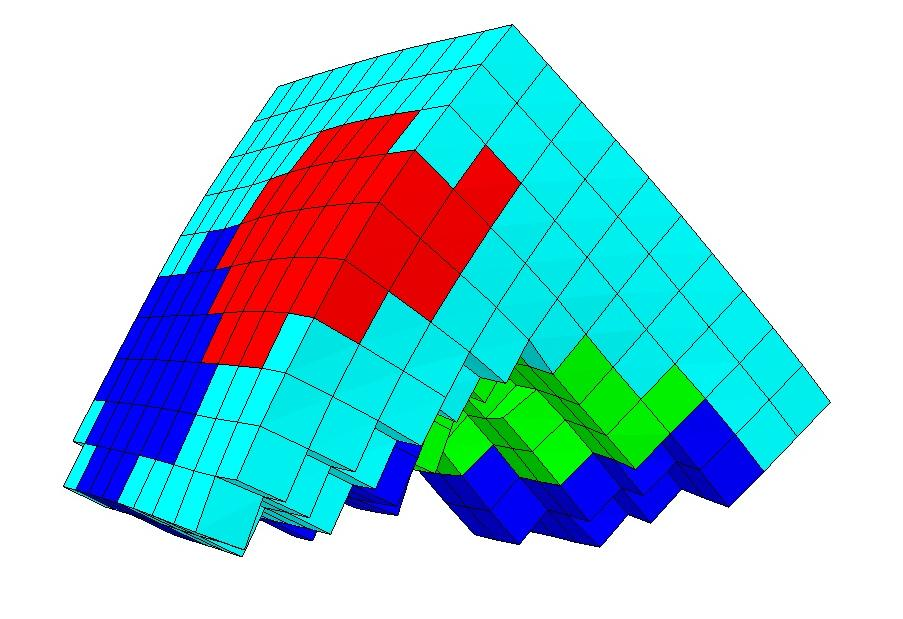
\includegraphics[height=0.2\textheight]{../Figures/Misc/allSoftMaterials.png}
\caption{Soft robot using four materials (two active, two passive), morphology evolved penalizing actuated materials.}
\label{fig:allSoftMaterials}
\end{figure}

Within the VoxCad simulation software there is the option of defining and using a palette of materials. Materials can be \emph{passive} or \emph{active}. Passive materials do not react to temperature changes, while active materials expand and contract in respect to their thermal properties. Figure~\ref{fig:allSoftMaterials} illustrates a soft robot consisting of all four materials are used in the experiments. \textcolor{Red}{Red} and \textcolor{Green}{Green} are the only actuated materials with non-zero and opposite thermal expansion coefficients, meaning that their phase in respect to the actuation from temperature changes is equal to half a circle. Green voxels contract the same time red expand and vice versa, mimicking living organisms' muscle tissue. The two additional materials represent soft non-actuated tissue that can be soft (soft tissue) or hard (bones). \textcolor{Cyan}{Cyan} voxels are soft having five times smaller elastic modulus of their material than \textcolor{Blue}{Blue} which have $50$ \texttt{MPa}.


\section{Random Generation of Soft Robots}

To evaluate all the following evolutionary methods used, information about the performance of random generated morphologies must be present. In order to achieve that, two random approaches which will also help the understanding between direct and indirect encoding are implemented. 

The first implementation of a random morphology generator mimics ``direct'' encoding. This method assigns randomly the presence of a voxel in the three-dimensional space of the lattice. The probability of adding a voxel in given coordinates is $0.5$. The material of each newly added voxel is chosen randomly from the material palette. Each material has the same probability of being chosen. After all voxels have been added and assigned a material, unconnected parts of of the structure will be removed keeping only the largest connected structure in the lattice.


\begin{figure}
\centering
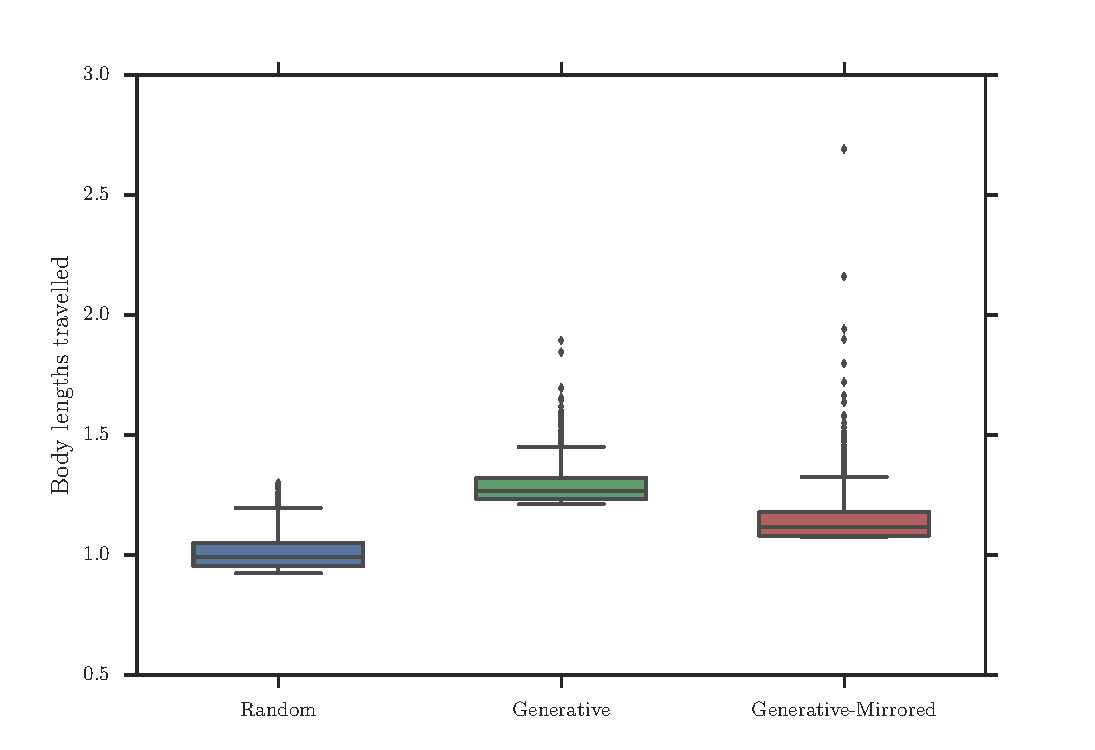
\includegraphics[width=1.0\textwidth]{../Figures/Results/random.pdf}\\
\hspace{0.1cm}
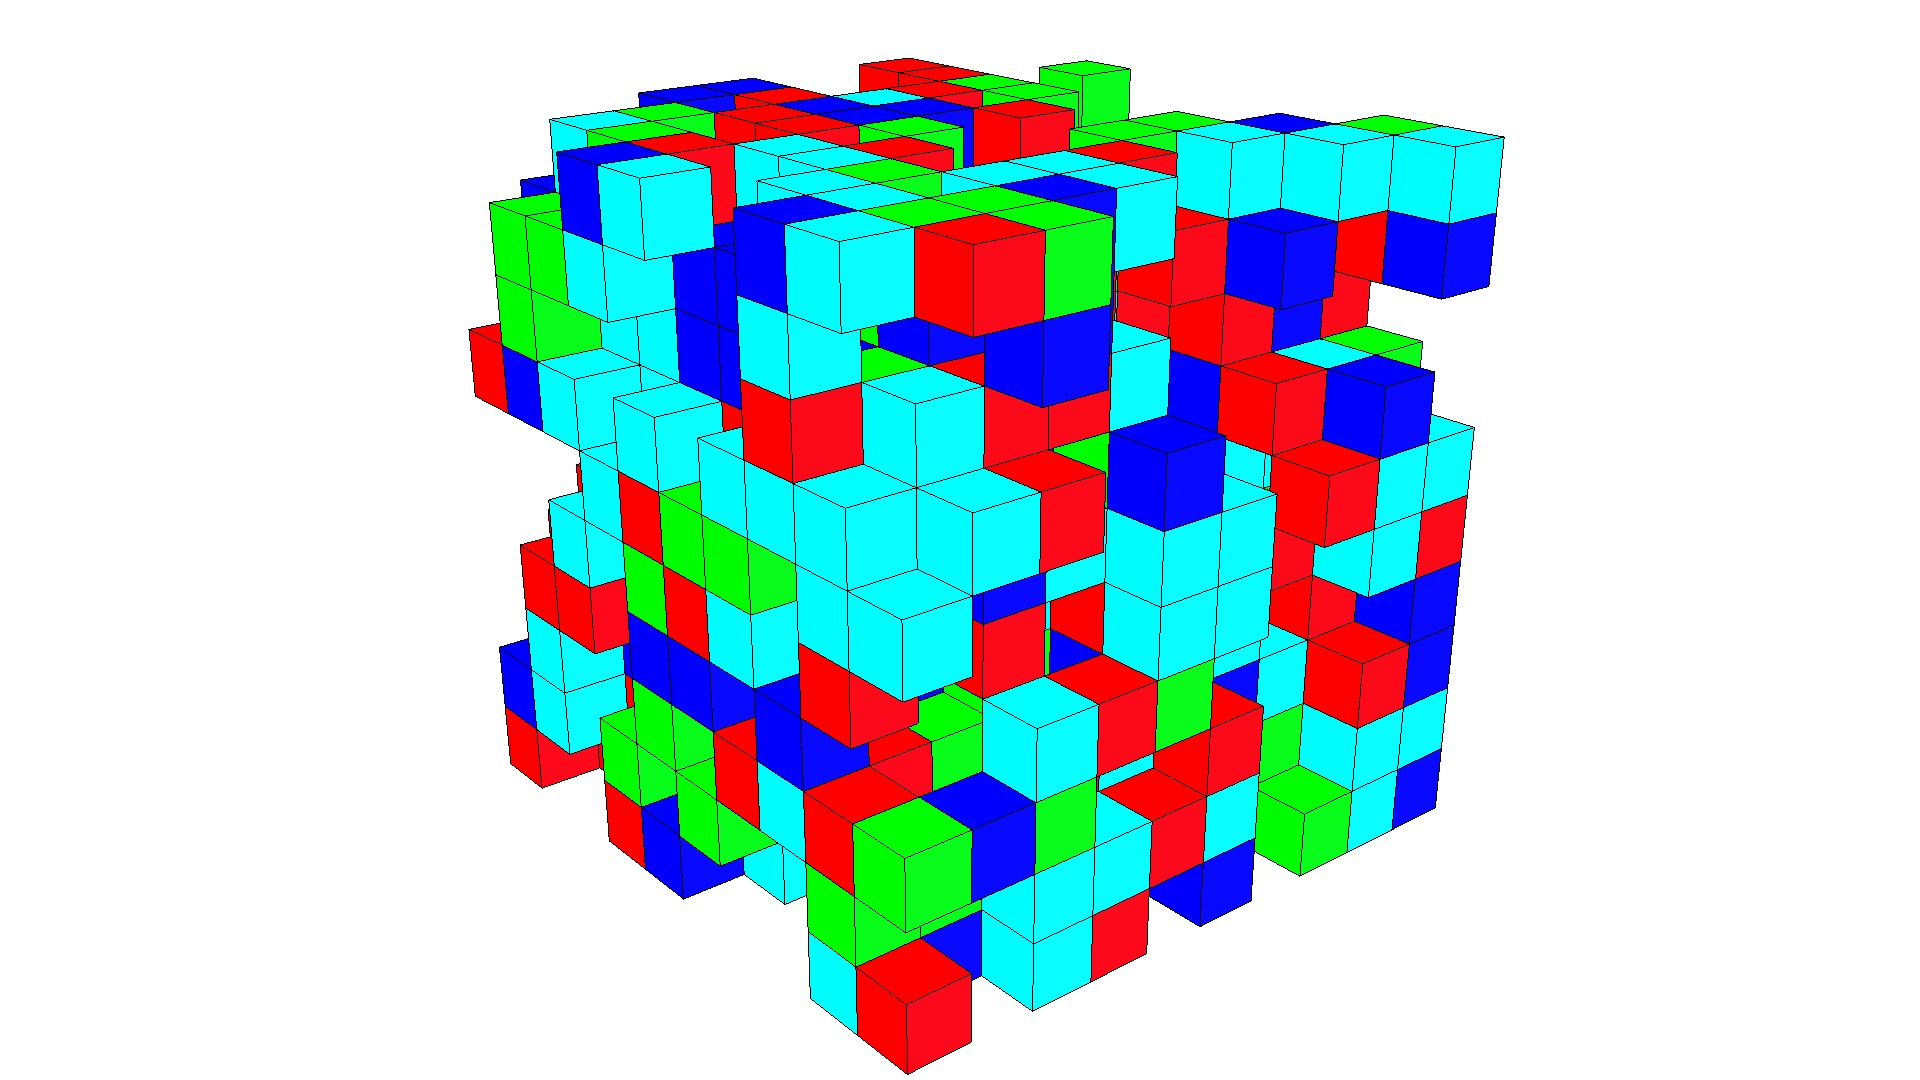
\includegraphics[height=0.15\textwidth]{../Figures/Robots/random.jpg}
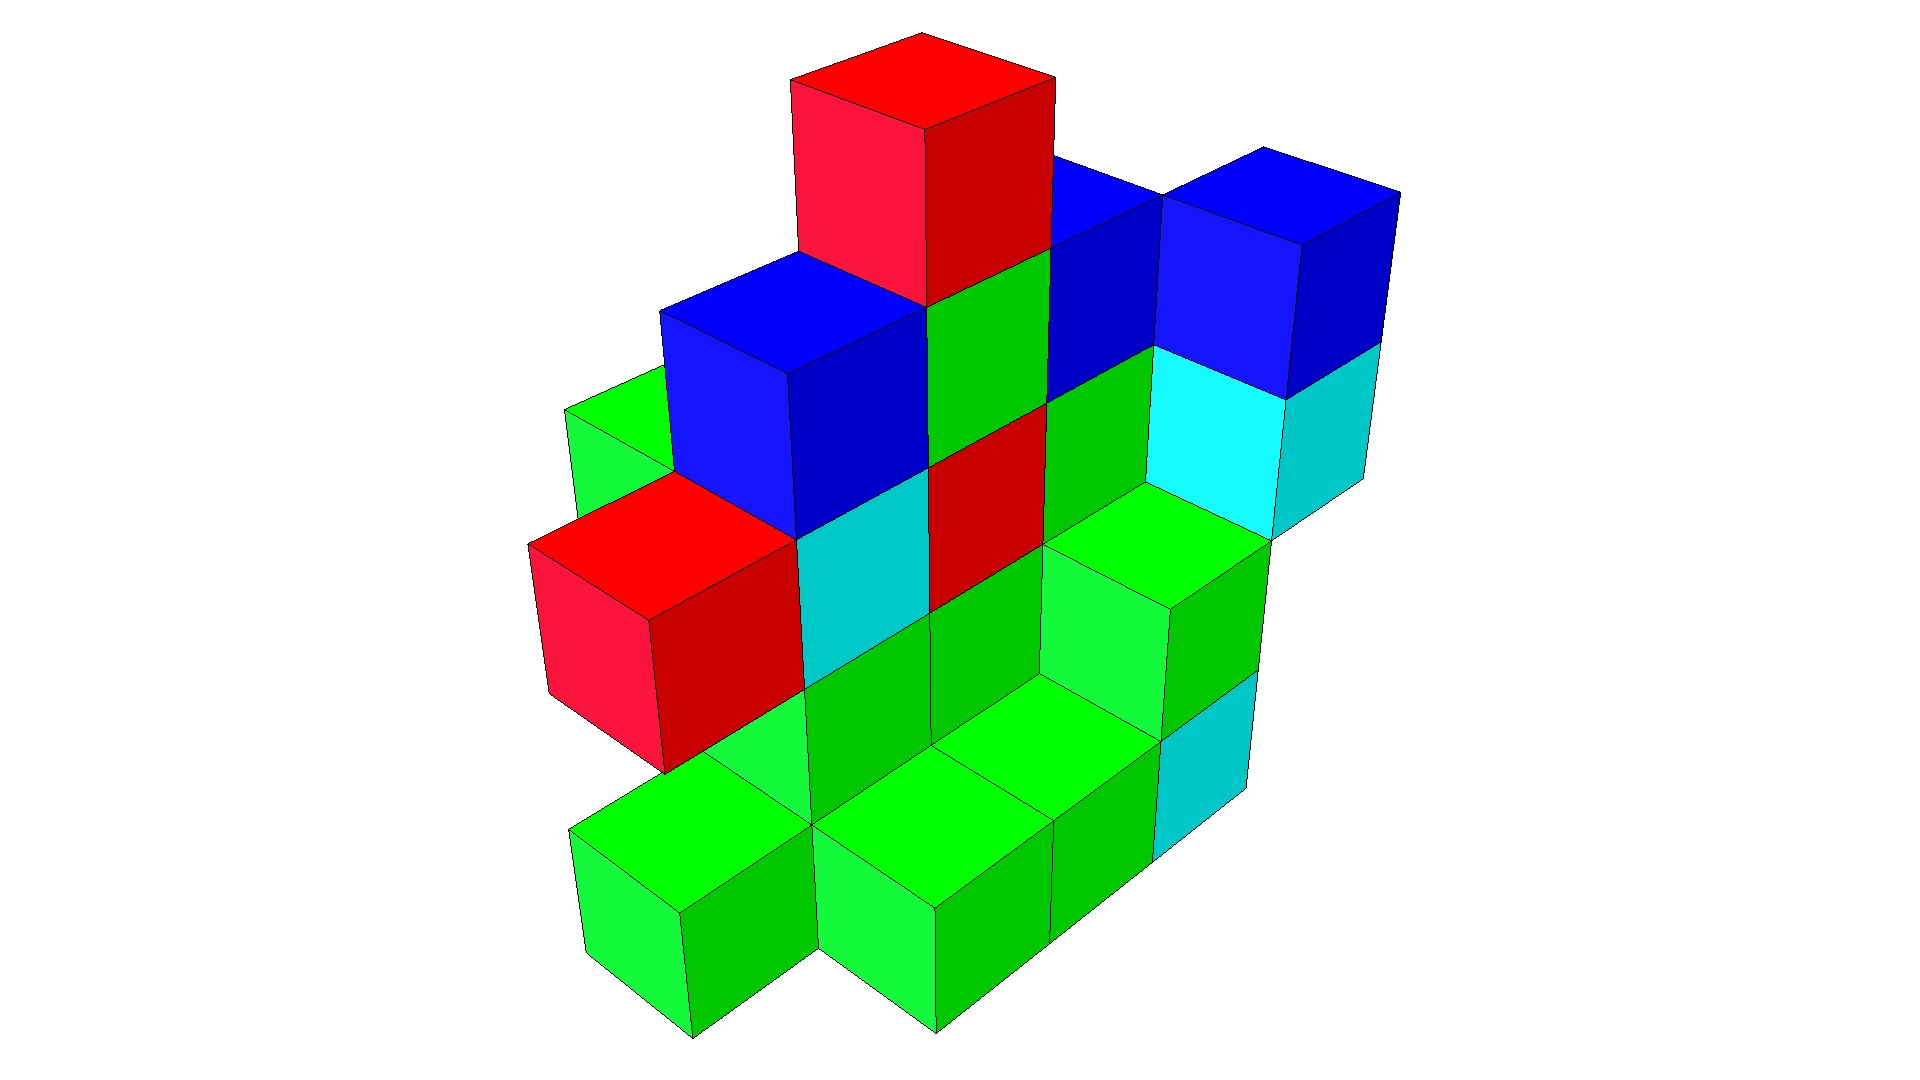
\includegraphics[height=0.15\textwidth]{../Figures/Robots/rg0.jpg}
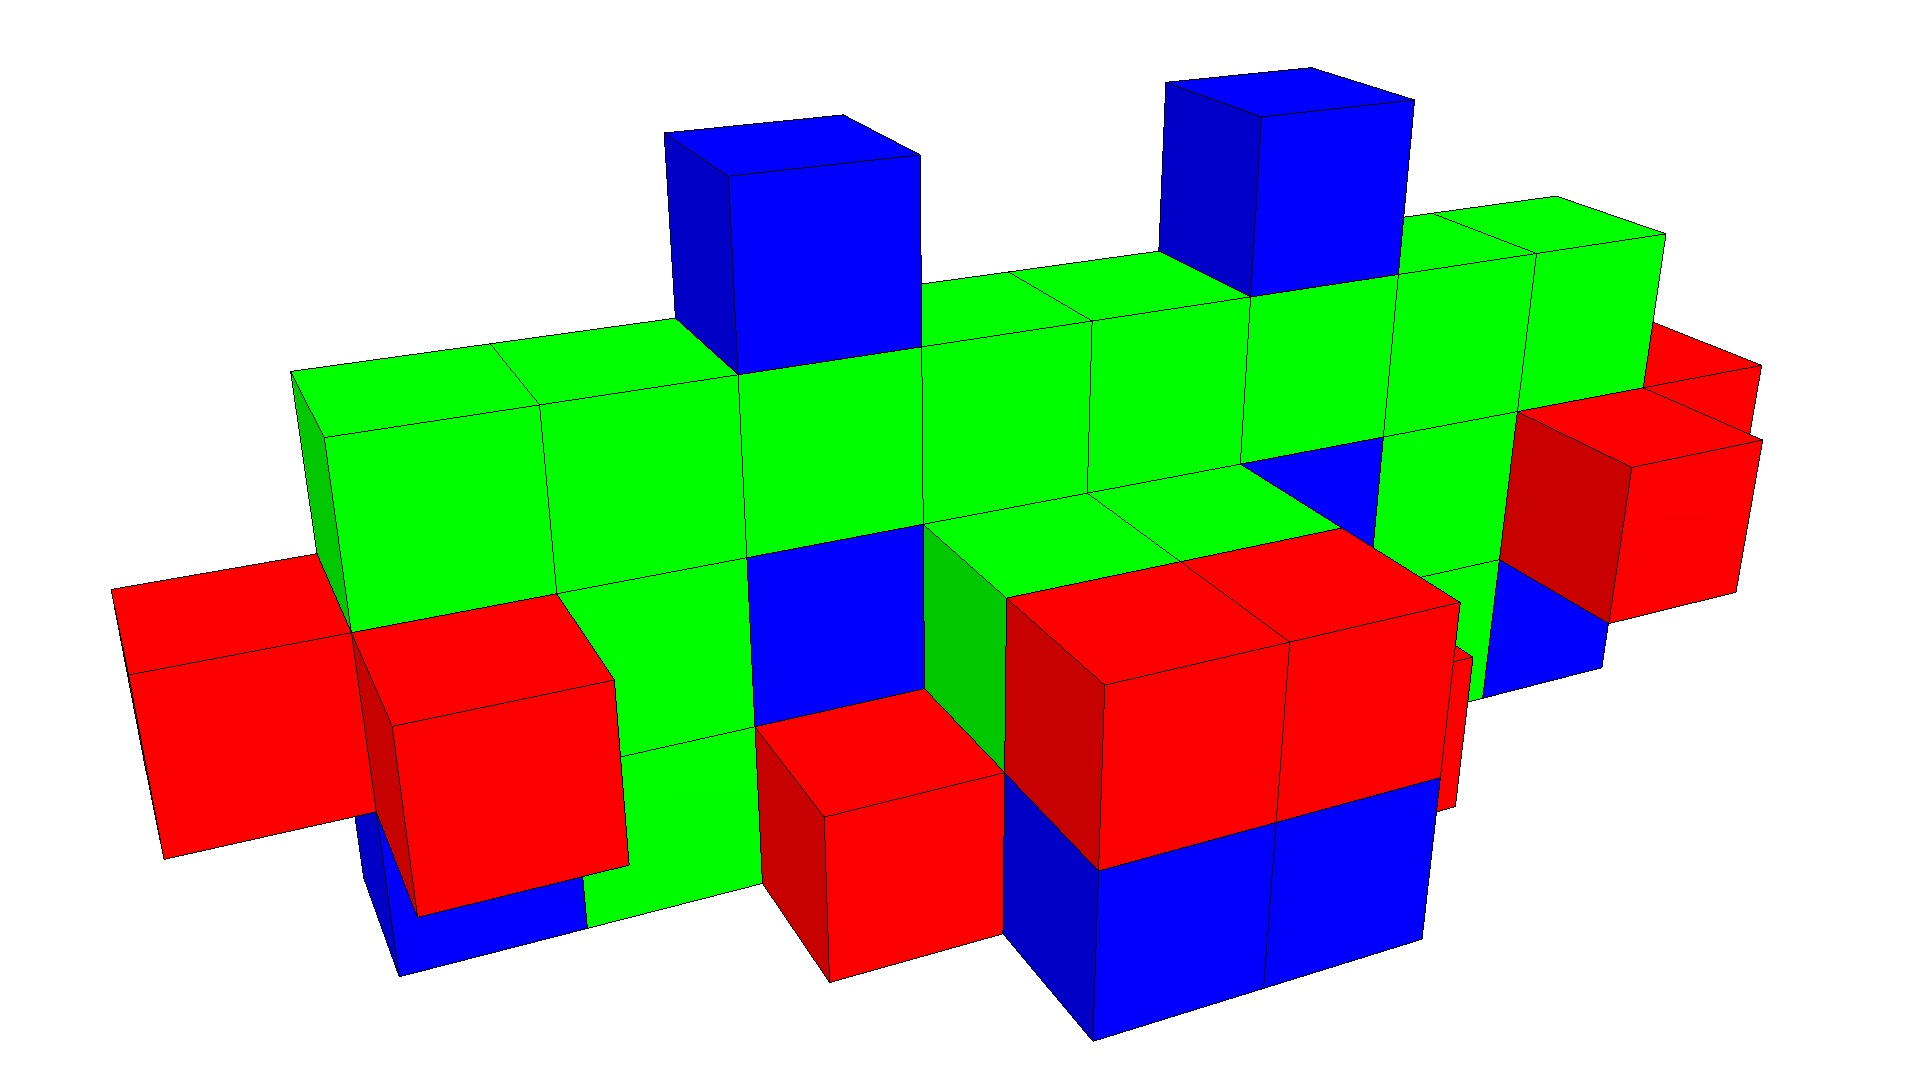
\includegraphics[height=0.15\textwidth]{../Figures/Robots/rg1.jpg}
\caption{Generative random approaches create more natural morphologies (see Settings~\ref{Settings-size10}).}
\label{fig:randomResultsRobots}
\end{figure}

An ``indirect'' way of generating random morphologies follows a different method of assigning materials to voxels, adopting a set of rules in order to generate a new soft robot morphology. This method holds two probabilities, the one refers to the probability of adding a new voxel in the already generated structure, the next one denotes the probability that the material of a new inserted voxel will be the same as the one of the material is going to be connected to. First, a random material voxel is inserted in a random coordinate into the lattice space. When a new voxel is to be added, a connection (voxel) is chosen from the already added voxels. The side of the connection is chosen from a uniform distribution out of all valid (within the lattice space) sides. In this generative process there is also the possibility of creating structures in half of the lattice space and then mirror the soft structures in both halves of it, generating in this way symmetrical morphologies.

Considering these three methods the difference between direct and indirect coding presented in section~\ref{DirectIndirect} is becoming easier interpreted. In the ``direct'' process a probability determines the presence and the material for every coordinate in the lattice space. On the other hand, the ``generative'' method holds a set of rules and probabilities defining the structure that is going to be produced in the available space.

Figure~\ref{fig:randomResultsRobots} illustrates not only the actual performance (fitness in body lengths traveled by top-$1000$ soft robots from $30000$ total runs for each method) of the previously described methods, but also one of the best performing soft robots of each method. Both ``generative'' methods outperform the ``direct'' one due to the fact that they are capable of generating regular morphologies. ``Generative'' random soft robot generation methods create more compact structures which can move easier due to their size and their geometrical features. For the \textit{Generative-Mirrored} approach even though the average performance is slightly worse than the plain method it actually performs way better in some distinct cases (i.e outliers). Adding geometrical properties resulted in getting more efficient locomotion by the generated soft robots.

All methods achieved an average displacement of the soft robots around or more than one body length, which is considered to be very low in respect to the robots generated by evolutionary methods are presented later in this thesis.

\section{Direct-Encoded Evolutionary Soft Robots}
\label{DirectEncodingEvolution}

\begin{figure}
\centering
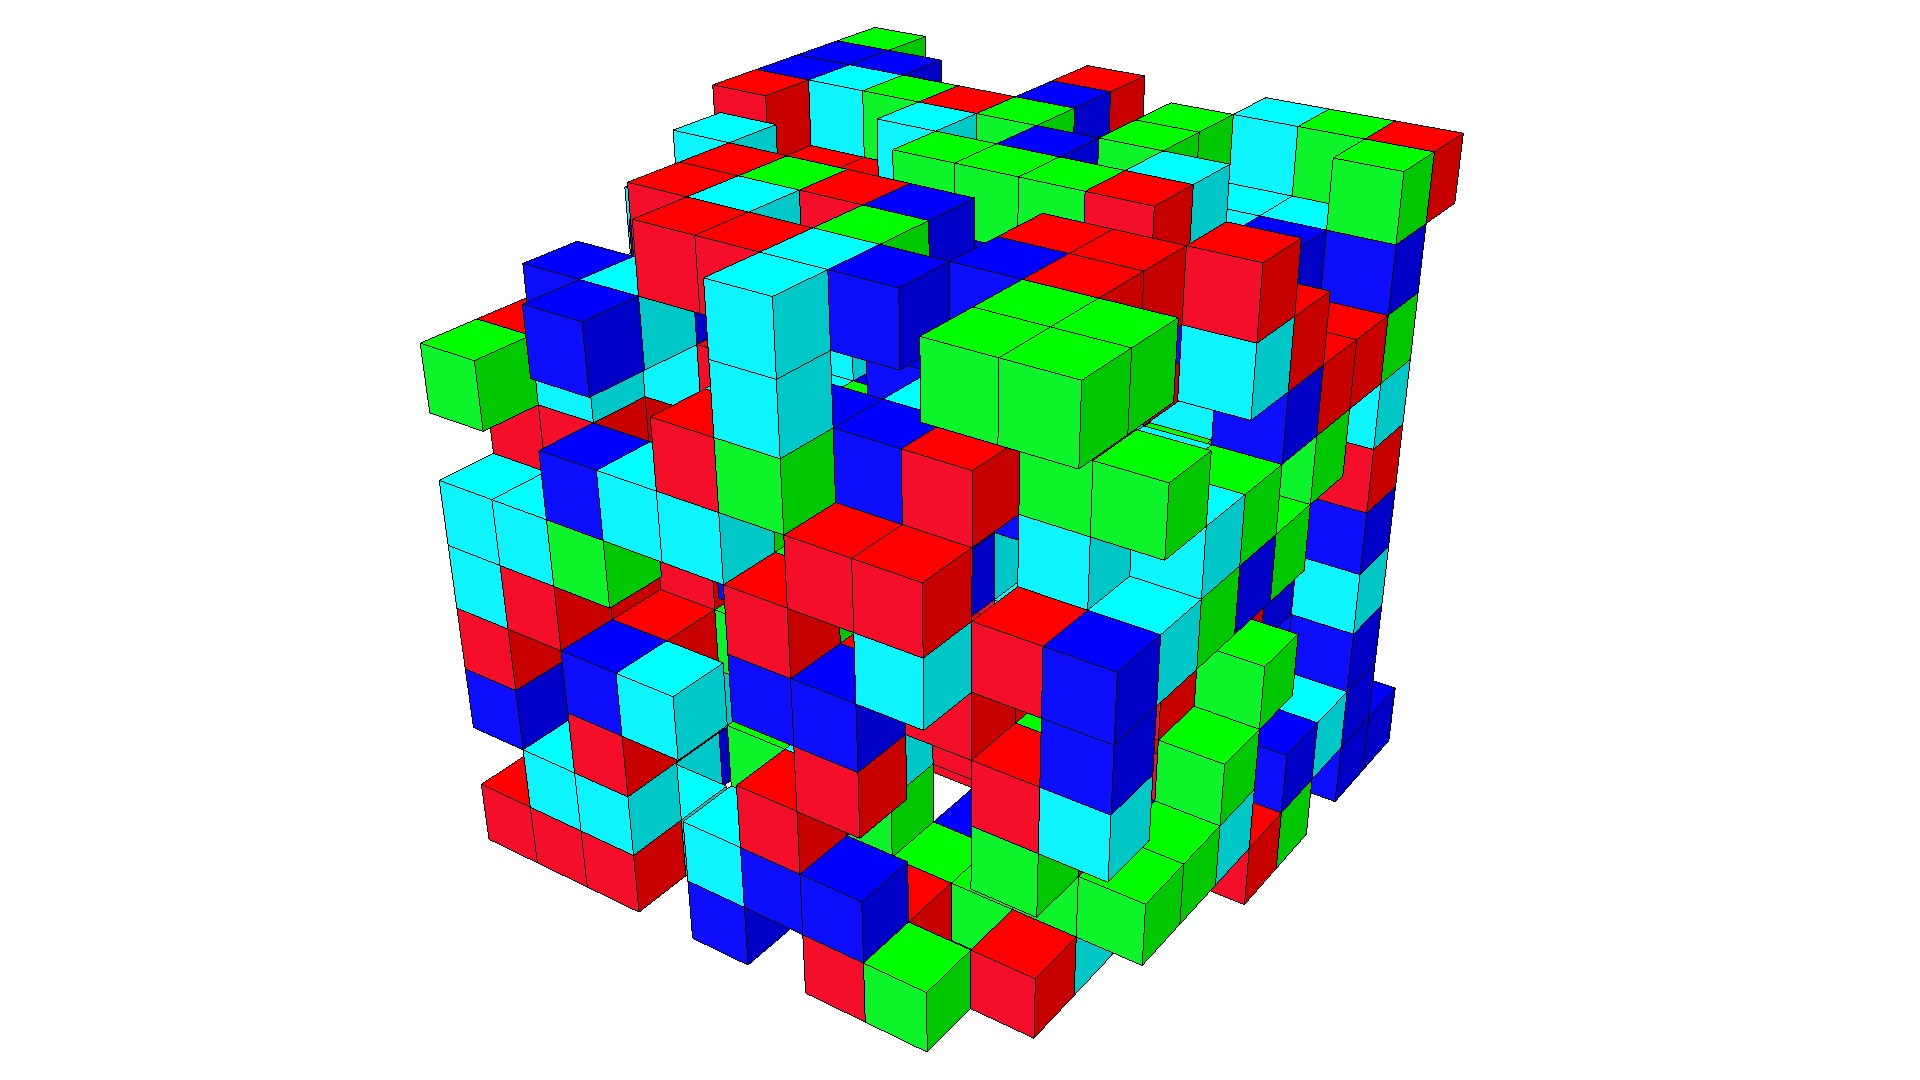
\includegraphics[height=0.2\textheight]{../Figures/Robots/direct.jpg}
\caption{Direct encoding cannot capture the geometrical properties of some problems.}
\label{fig:directRobot}
\end{figure}

In the previous section three random methodologies of ``indirect'' and ``direct'' generation of soft robots were implemented, failing to produce any decent locomotion gaits for the soft structures. Considering how vast the solution space is, random approaches are doomed to fail in a definite number of tries. Therefore, a more sophisticated evolutionary method is discussed here.

Direct encoded genomes coupled with a simple genetic algorithm is a successful approach in evolving robot controllers. As it was previously stated in Chapter~\ref{Background}, mutations and crossovers of real-value streams search the problem space effectively finding near optimal solutions in demanding optimization problem domains. The GAlib C++ library \citep{wall1996galib} is used for the implementation of this method.

\paragraph*{Representation of the genotype}~\\
As in every direct encoding scheme genotype is represented by a stream of bits, which length is equal to the number of dimensions of the problem. The number of the materials in the palette are the first dimensions of the problem. The presence or not of a voxel at a given position in the lattice space adds one more dimension to the representation. Analytically, its length can be represented by a stream of length equal to the number of voxels in the lattice times the materials used plus one denoting the presence of the voxel, the length of the genome is described by the following equation:
\begin{equation}
\label{lengthDirect}
| Genome | = (l_x \times l_y \times l_z ) \times (1 + |p|)
\end{equation}
where $l_x, l_y, l_z$ are the dimensions of the lattice space, and $|p|$ is the size of the palette of materials.
\begin{equation*}
Genome = \underbrace{01010\ldots011011}_\text{Presence}\ \    \underbrace{10101\ldots110011}_{Material_1} \   \ldots\  \underbrace{00011\ldots111110}_{Material_n}
\end{equation*}
The above stream of bits illustrates how a soft structure in VoxCad environment can be represented by a direct encoding scheme. Each of the values of the stream is represented by a float value between zero and one, which is represented by a stream of bits in lower-level. The mapping from the genotype level to the phenotype is straightforward in this case, the first stream of values is used to determine the presence of a voxel in given coordinates while in case of presence the other $n$ streams are used and the maximum value in specific positions of the streams determine the material is going to be used.

Considering the representation of the genome, as well as the geometrical nature of the problem itself it is not expected that direct encoding will capture this major property of the problem (see Fig.~\ref{fig:directRobot}). Therefore, it is anticipated that direct encoded genomes will not be able to generate soft robots that can produce efficient locomotion in these settings~\citep{cheney2013unshackling}.





\section{Generative-Encoded Evolutionary Soft Robots}

Direct encoding methods lack the morphology regularities of the soft robots evolved by this method. Compositional pattern-producing networks can serve this function. CPPNs are built up by a set of canonical functions which enable the outputs of the network to produce repetitive, symmetrical and geometrically interesting patterns. Producing regularities in the phenotype space and capturing geometrical properties of the optimization problem, it is expected that this representation is going to produce efficient locomotion strategies and morphologies of the soft structures~\citep{cheney2013unshackling}.
\begin{figure}
\centering
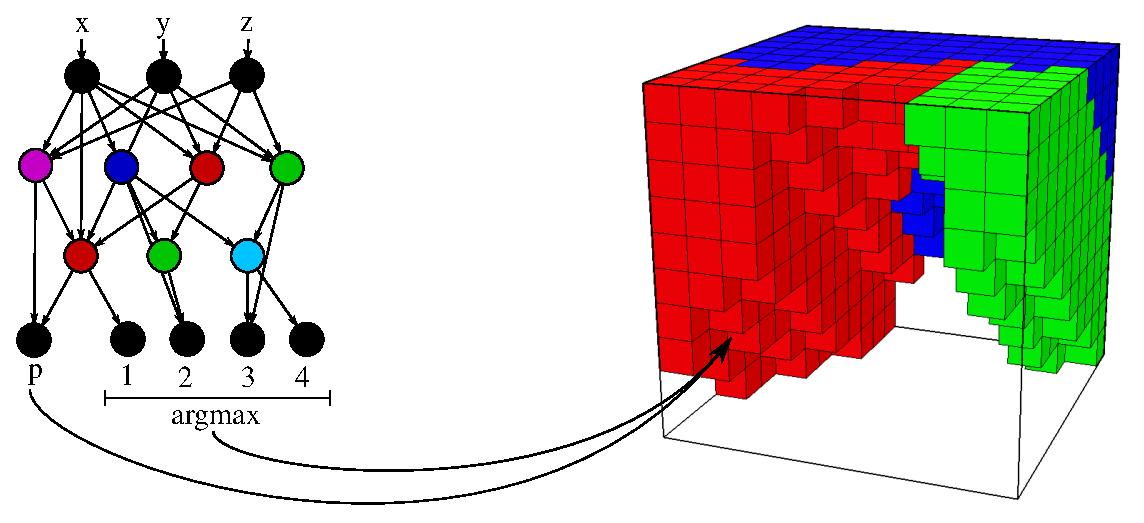
\includegraphics[height=0.2\textheight]{../Figures/Misc/cppnSoftBot.eps}
\caption{Each genotype (CPPN) is queried for every coordinate inside the lattice space, its outputs determine the presence of a voxel and the type of its material.}
\label{fig:cppnDiagram}
\end{figure}
Since, CPPNs must be queried for every coordinate of the lattice space, the input nodes (neurons) of the CPPN are assigned to x,y,z normalized coordinates following~\citep{cheney2013unshackling}, so that:
\[x,y,z \in [-1,1]\]
A bias input node is also introduced in the genome CPPN representation, this will allow the network to produce arbitrary outputs different from the defaults when all other inputs values are set to zero. More inputs could be added to the CPPNs, for instance the distance from the center point of the Cartesian phenotype space (lattice) as described in~\citep{stanley2007compositional} and used in~\citep{cheney2013unshackling}, which naturally adds more bias towards symmetrical structures. However, the evolution of such aesthetic structures is not much of interest to exploit. CPPNs, as it is shown later in this thesis, can evolve symmetrical morphologies without this extra information input node(s). The proposed input nodes for the three dimensions of the Cartesian space provide the minimum bias to the network outputs. Figure~\ref{fig:cppnDiagram} illustrates the topology of a random CPPN network with the input and output nodes previously described. The set of nodes and connections determine the \emph{topology} of the network. The topology of these networks can be variant and be evolved alongside the weights of the connections in any neuroevolution method. The divergent part of the network between the input and the output nodes is described by the genotype and it is the one that is going to be evolved and altered during the evolution. The presence of a voxel in each coordinate of the lattice is determined by a single output of the CPPN, denoted with $p$ while the selection of the material is determined by $n$-outputs. The node with the maximum value out of the $n$-outputs will determine which of the materials is going to be used in the specific voxel only in cases this is present.

\subsection{Evolution of Generative Encoded Genomes}

The evolution of these indirect representations of the genotypes can be evolved with any method able to evolve artificial neural networks, since these are identical to CPPNs. CPPN-NEAT (see Sec.~\ref{CPPN}), is a method to evolve CPPNs with the NEAT evolutionary method. Previous work~\citep{cheney2013unshackling}, showed that this method can indeed evolve the morphologies of the soft robots in the VoxCad simulation environment. \textit{HyperNEAT}\footnote{HyperNEAT \texttt{v4.0 C++} by J. Gauci code (url: \url{https://github.com/MisterTea/HyperNEAT})} is used for the implementation of the CPPN-NEAT algorithm. Algorithm~\ref{evolutionPseudocode}, presents the pseudocode for the evolution under CPPN-NEAT method. In addition, a brief explanation of the function used in the algorithm follows:


\begin{algorithm}[t!]
\caption{CPPN-NEAT evolution}
\label{evolutionPseudocode}
\begin{algorithmic}[1]
\STATE $\mathtt{population} = \varnothing$
\STATE $\mathtt{species} = \varnothing$
\STATE $\mathtt{generation}[0] = \mathbf{initial\_population}()$
\FOR{ $i = 0\   \text{to}\  \mathtt{max\_generation}$}
\STATE $\mathtt{species} = \mathtt{species} \cup \mathbf{speciation}(\mathtt{generation}[i])$
\STATE $\mathbf{evaluation}(\mathtt{generation}[i])$
\STATE $\mathbf{adjust\_fitness}(\mathtt{generation}[i], \mathtt{species})$
\STATE $\mathbf{selection}(\mathtt{generation}[i], \mathtt{species})$
\STATE $\mathtt{generation}[i+1] = \mathbf{reproduction}(\mathtt{generation}[i])$
\STATE $\mathtt{population} = \mathtt{population} \cup \mathtt{generation}[i+1]$
\ENDFOR
\end{algorithmic}
\end{algorithm}

\begin{description}
\item[Initial population]{Before the evolution starts, an initial population must be produced, identical genomes (CPPNs), with variant connection weights fill up the population.}

\item[Speciation]{Takes place and split the population in separate species or adds individuals to already existing species in respect to their networks' topologies; a compatibility function determines the similarity between two genomes (see Eq.~\ref{CompatibilityEquation}). However, all firstly introduced genomes belong to the same species, due to the identical topology of their CPPNs.}

\item[Evaluation] Once the population is filled with new individuals, these have to be evaluated. Simulation is taking place for each of the individuals of the population, where each one of them is awarded with a fitness value.

\item[Fitness adjustment]{After all individuals are evaluated, each species is assigned a value which is the sum of the fitness values of the individuals belonging to this species divided by the number of the individuals. This way, it is been decided how many individuals each of the species will breed and it is directly determined by the average fitness of each species.}

\item[Selection]{As soon as the number of new individuals each species is determined, only the top $20\%$ of the species population will reproduce, the rest population will ``die''. \emph{Competition}, and \emph{Elitism} as other genetic selection techniques can also be used in this step of the evolution.}

\item[Reproduction]{There are two ways for the selected individual inside each species to reproduce. These are \emph{mutation}, which slightly changes the genome of one parent to create a new genome, and \emph{crossover}, where two parents combine their genes to create a new individual.}
\end{description}






\subsection{Novelty Search}

Novelty search, as first presented in Chapter~\ref{Background}, requires only small changes in the pipeline of an evolutionary algorithm. Fitness is replaced by a novelty metric which determines how novel is a phenotype's observed behavior with respect to all novel behaviors found earlier in the evolution. Sparsity (see Eq.~\ref{sparsenessEquation}) is used to determine this value while every individual is compared not only with the previous novel behaviors, but also with the observed behaviors by individuals from the current generation.
\begin{algorithm}[t!]
\caption{CPPN-NEAT with \textcolor{BrickRed}{novelty search}}
\label{noveltyPseudocode}
\begin{algorithmic}[1]
\STATE $\mathtt{population} = \varnothing$
\textcolor{BrickRed}{\STATE $\mathtt{novel\_inds} = \varnothing$}
\STATE $\mathtt{species} = \varnothing$
\STATE $\mathtt{generation}[0] = \mathbf{initial\_population}()$
\FOR{ $i = 0\   \text{to}\  \mathtt{max\_generation}$}
\STATE $\mathtt{species} = \mathtt{species} \cup \mathbf{speciation}(\mathtt{generation}[i])$
\STATE $\mathbf{evaluation}(\mathtt{generation}[i])$
\textcolor{BrickRed}{
\FORALL {$\mathtt{ind} \in \mathtt{generation}[i]$}
\STATE $\mathtt{novelty} = \mathbf{sparsity}(\mathtt{ind}, (\mathtt{generation}[i] - \mathtt{ind}) \cup \mathtt{novel\_inds})$
\IF {$(\mathtt{novelty} \geq \mathtt{novelty\_{threshold}}\ ||\ \mathtt{novel\_inds} == \varnothing)$}
\STATE $\mathtt{novel\_inds} = \mathtt{novel\_inds} \cup \mathtt{ind}$
\ENDIF
\ENDFOR
\STATE $\mathbf{adjust\_novelty}(\mathtt{generation}[i], \mathtt{species})$
}
\STATE $\mathbf{selection}(\mathtt{generation}[i], \mathtt{species})$
\STATE $\mathtt{generation}[i+1] = \mathbf{reproduction}(\mathtt{generation}[i])$
\STATE $\mathtt{population} = \mathtt{population} \cup \mathtt{generation}[i+1]$
\ENDFOR
\end{algorithmic}
\end{algorithm}
The algorithmic adjustments within CPPN-NEAT algorithm are indicated in Algorithm~\ref{noveltyPseudocode} (\textcolor{BrickRed}{Red} colored text), where the pseudocode of novelty search is presented.

\textbf{Evaluation} function in fitness based evolution was responsible of evaluating an individual in respect to an objective. This objective function is equal to the body-lengths traveled by the soft robot within a specific time span. However, the same function is now also responsible for observing the behavior of each individual and record it. In this way, the novelty of a behavior can be computed based on recorded behaviors of other individuals. Function \textbf{sparsity} computes the sparseness (see Eq.~\ref{sparsenessEquation}) of a specific individual's observed behavior in the behavior space. Following the evaluation of each individual, its behavior will be compared to all novel behaviors stored during the evolution. A threshold determines if the observed behavior is considered novel in respect to the set of behaviors was compared to. The fitness adjustment of the previous code example is becoming \textbf{novelty adjustment} following the same functionality, selection and reproduction operations can be applied in the same way.


\subsubsection{Behavior in novelty search}
\label{BehaviorNoveltySearch}

\begin{table}
\centering
\caption{Observed soft robot behaviors used for the sparsity computation in novelty search.}
\label{Behaviors}
    \begin{tabular}{lrcc p{4cm}}
    \toprule
    \textbf{Behavior} &
    \textbf{Sampling} &
    \textbf{DFT} &
    \textbf{Example} &
    \textbf{Description} \\
    \midrule
    \Vcentre{3D-trajectory}    &
    \Vcentre{1 KHz}     &                       &
    \Vcentre{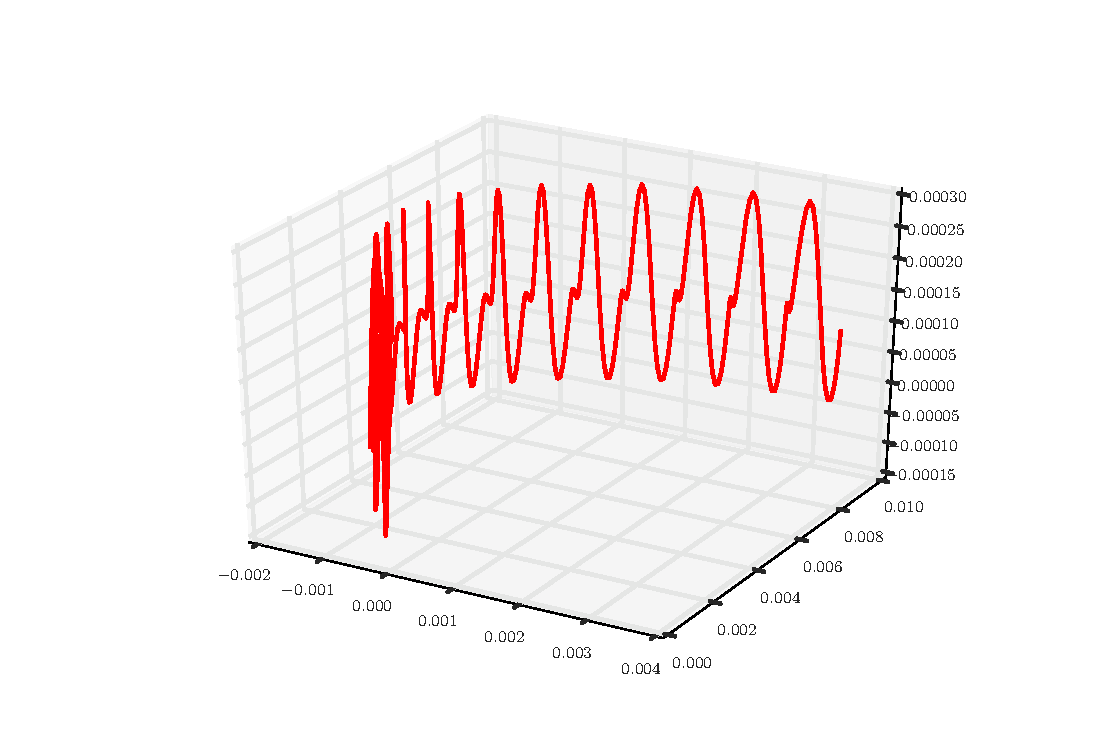
\includegraphics[scale=0.19]{../Figures/Behaviors/3d.pdf}} &
    \vspace{-.85cm}Set of three-dimensional sampled points of the robot's center of mass during simulation.  \\
    \Vcentre{2D-trajectory}   &
    \Vcentre{1 KHz}     &                     &
    \Vcentre{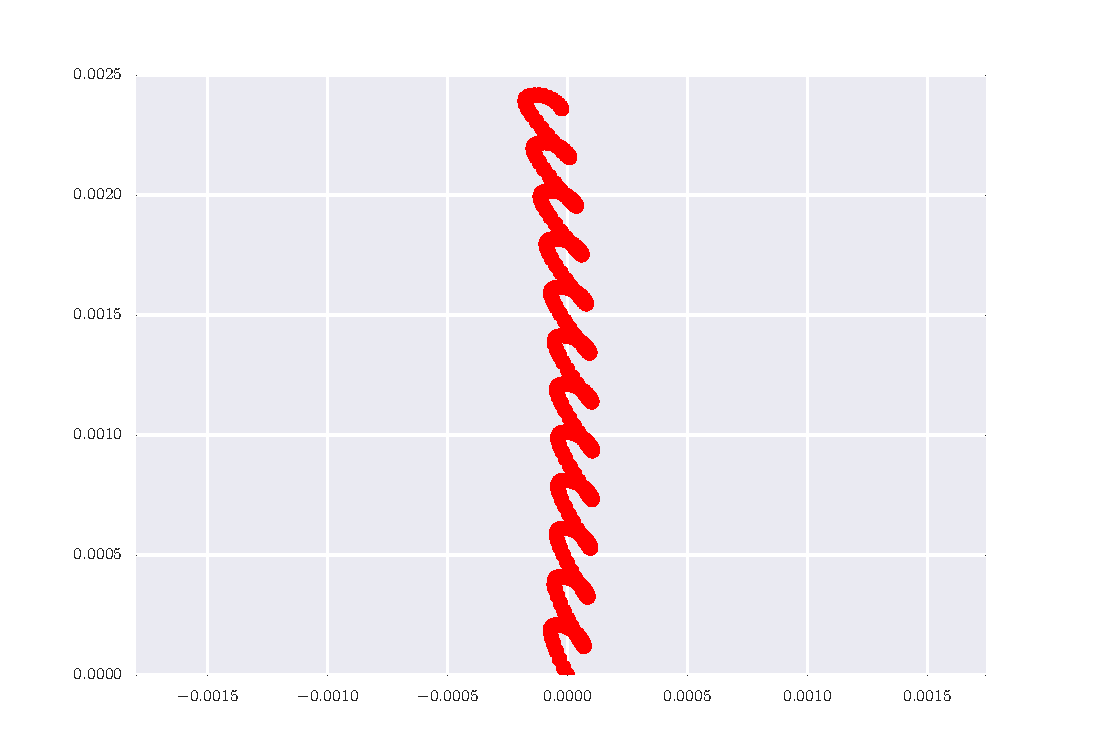
\includegraphics[scale=0.18]{../Figures/Behaviors/2d.pdf}} &
    \vspace{-.85cm}Set of two-dimensional ground projection sampled points of the robot's center of mass during simulation.      \\
    \Vcentre{Pace}                 &
    \Vcentre{1 KHz}     &                     &
    \Vcentre{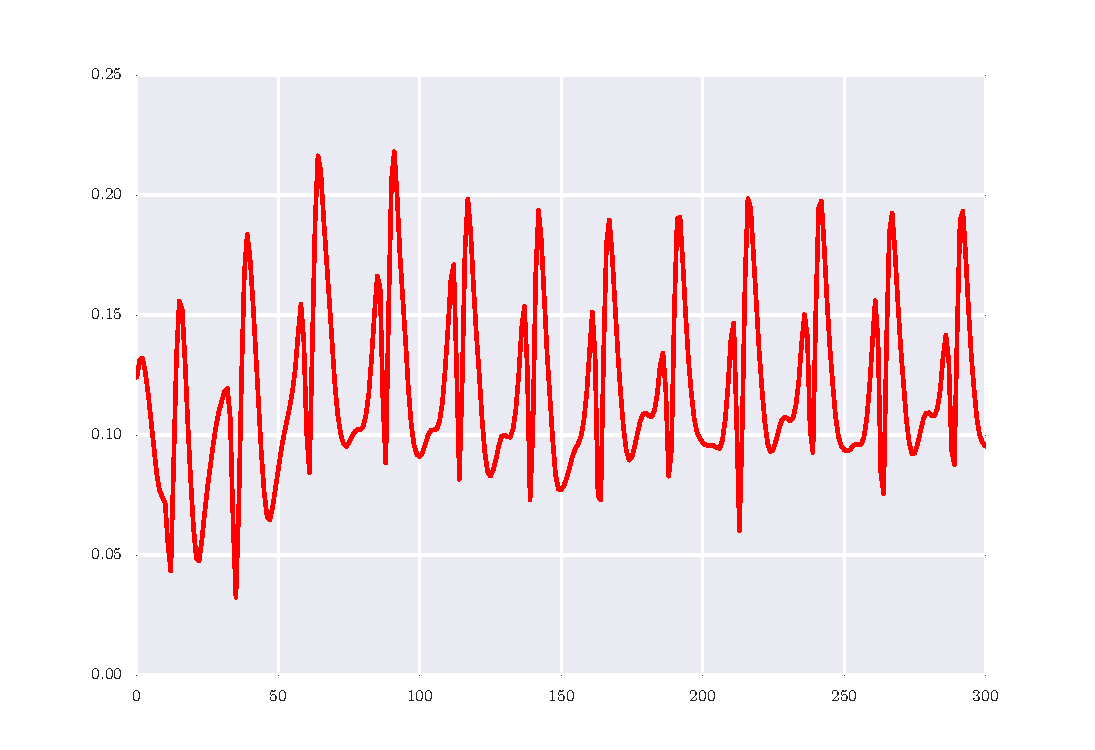
\includegraphics[scale=0.18]{../Figures/Behaviors/pace.pdf}} &
    \vspace{-.85cm}Set of robot's pace sampled values.    \\
    \Vcentre{DFT-Pace}             &
    \Vcentre{100 KHz}   &
    \Vcentre{\checkmark}                &
    \Vcentre{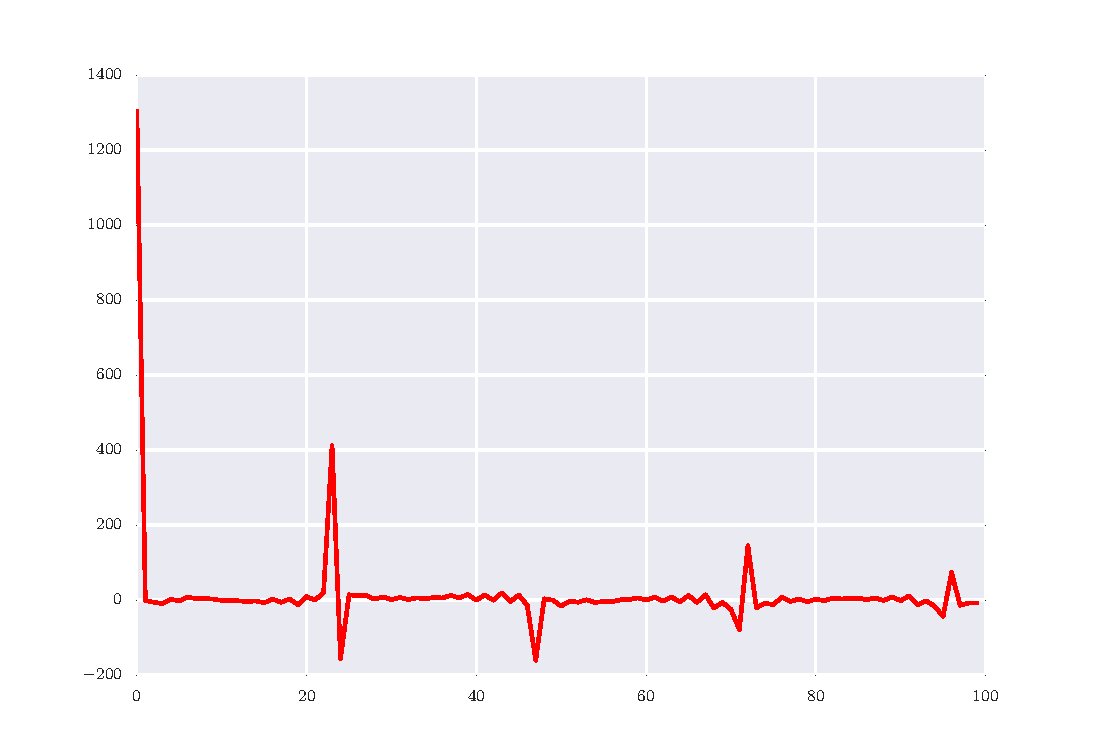
\includegraphics[scale=0.18]{../Figures/Behaviors/pacedft.pdf}} &
    \vspace{-.9cm}Set of the robot's pace sampled values transformed into the frequency space.    \\
    \Vcentre{VTG}                  &
    \Vcentre{1 KHz}     &                     &
    \Vcentre{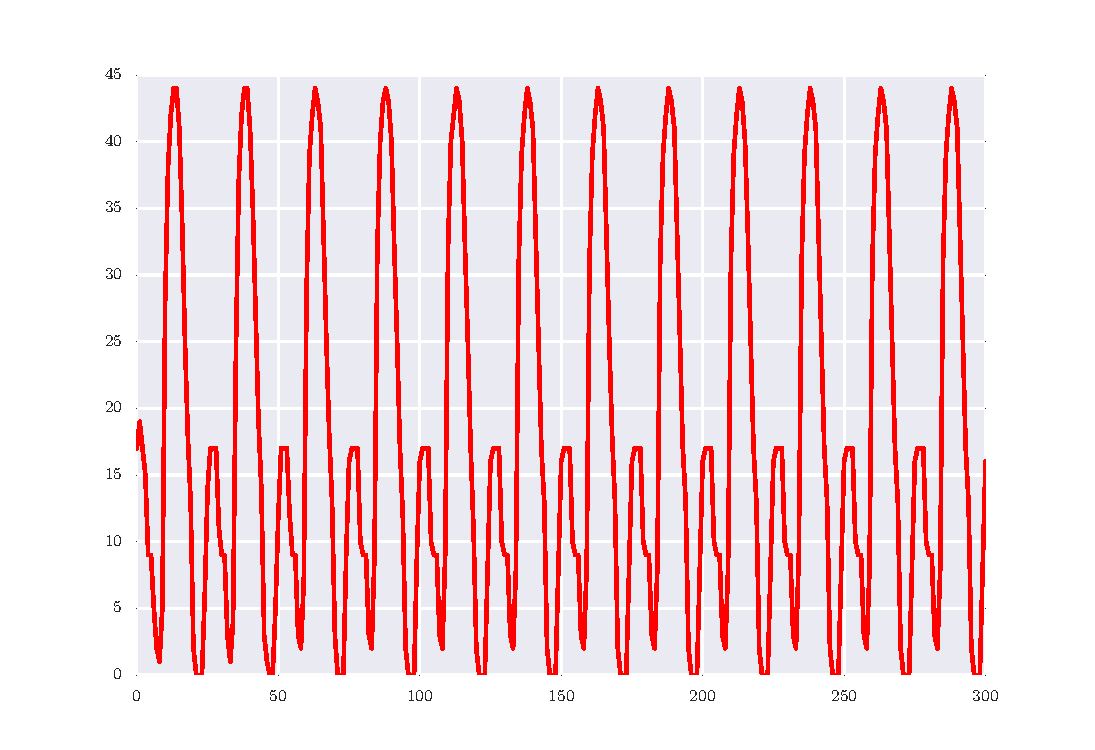
\includegraphics[scale=0.18]{../Figures/Behaviors/vtg.pdf}} &
    \vspace{-.85cm}  Set of voxels touching the ground in each sampling time.  \\
    \Vcentre{DFT-VTG}              &
    \Vcentre{100 KHz}   &
    \Vcentre{\checkmark}              &
    \Vcentre{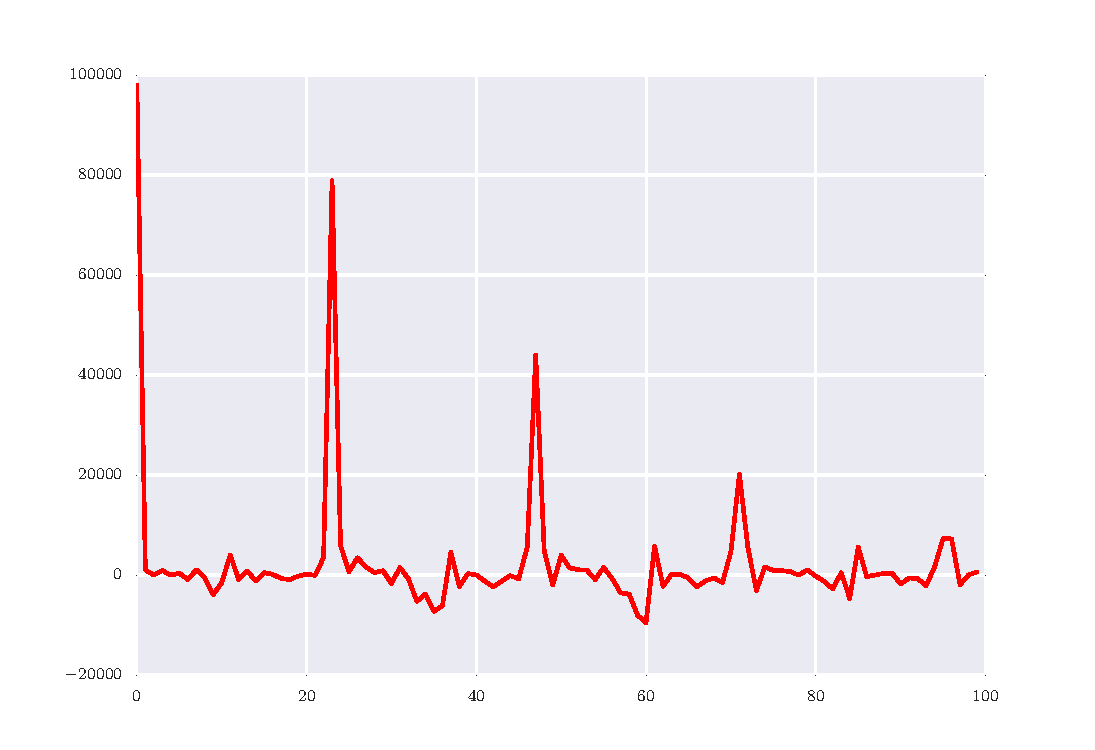
\includegraphics[scale=0.18]{../Figures/Behaviors/vtgdft.pdf}} &
    \vspace{-.85cm} Set of voxels touching the ground transformed into the frequency space.   \\
    \Vcentre{Pressure}             &
    \Vcentre{1 KHz}     &                     &
    \Vcentre{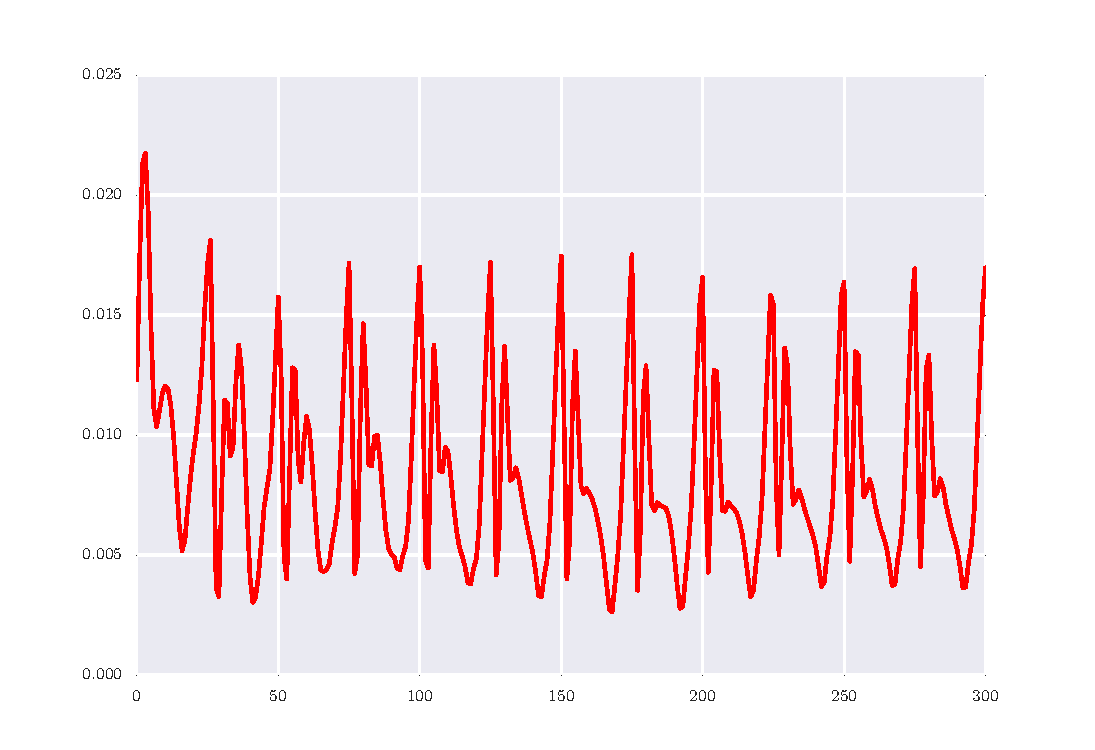
\includegraphics[scale=0.18]{../Figures/Behaviors/pr.pdf}} &
    \vspace{-.85cm} Set of maximum pressure among the connected voxels.  \\
    \Vcentre{DFT-Pressure}         &
    \Vcentre{100 KHz}   &
    \Vcentre{\checkmark}                &
    \Vcentre{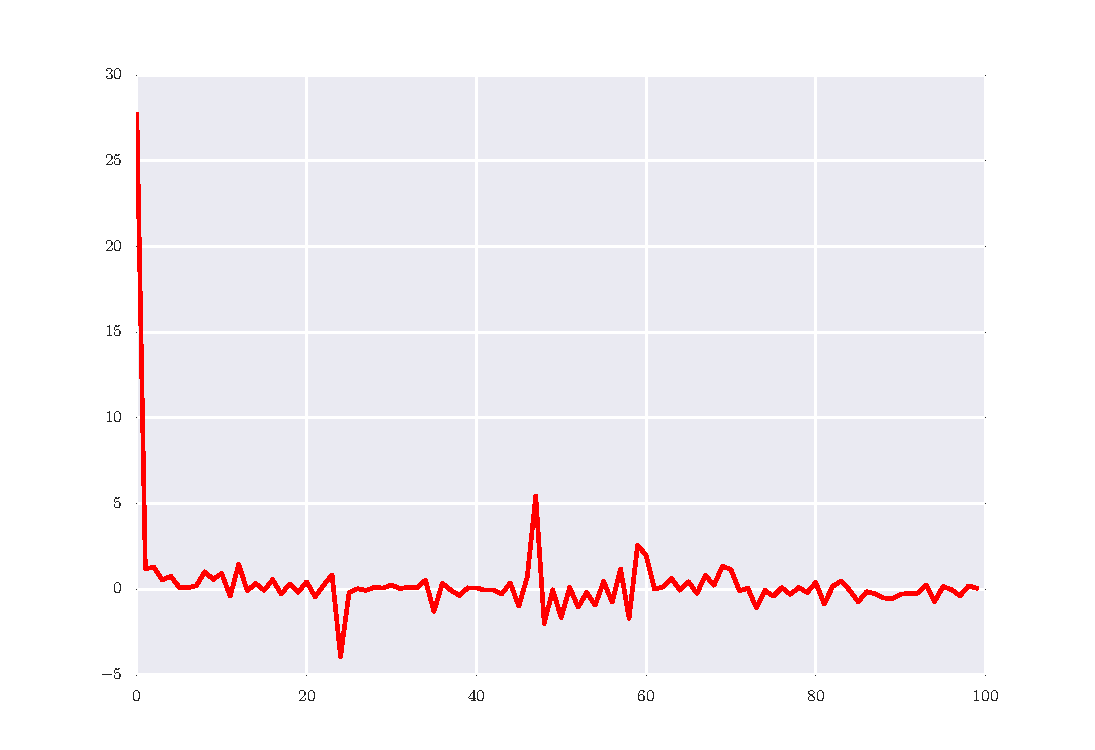
\includegraphics[scale=0.18]{../Figures/Behaviors/prdft.pdf}} &
    \vspace{-.85cm}Set of maximum pressure among the connections transformed into the frequency space.    \\
    \Vcentre{KE}                   &
    \Vcentre{1 KHz}     &                     &
    \Vcentre{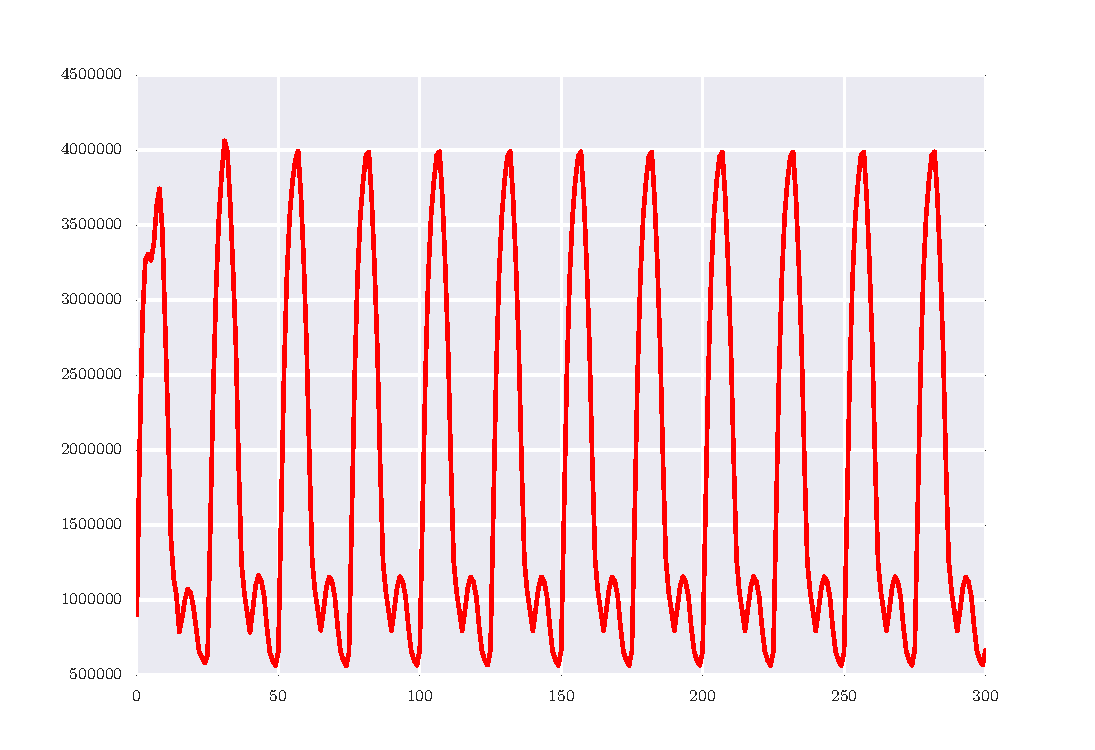
\includegraphics[scale=0.18]{../Figures/Behaviors/ke.pdf}} &
    \vspace{-.85cm}Set of maximum kinetic energy of voxels.    \\
    \Vcentre{DFT-KE}               &
    \Vcentre{100 KHz}   &
    \Vcentre{\checkmark}                &
    \Vcentre{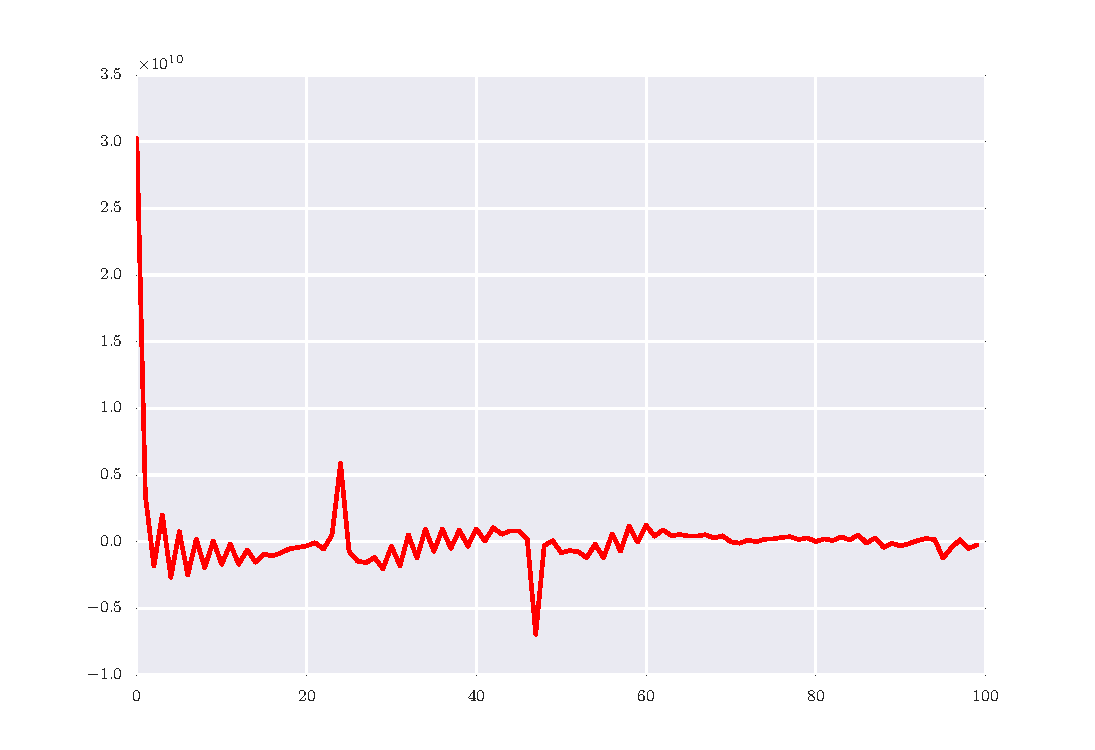
\includegraphics[scale=0.18]{../Figures/Behaviors/kedft.pdf}}  &
    \vspace{-.85cm}Set of maximum kinetic energy of voxels transformed into the frequency space.    \\
    \bottomrule
    \end{tabular}
\end{table}

\emph{Behavior} can be defined as the way that a human/machine behaves towards or within an environment. Regarding the evolution of soft robots in the specific simulated environment, a behavior can be defined as the way soft robots behave in respect to their locomotion strategy. Every aspect of the soft robots movement that can be observed can be used to describe their behavior. Previous work~\citep{lehman2011evolving} in a try to evolve walking three-dimensional virtual creatures used the evolved morphology of the creatures to describe their behavior. Although, in this work comparing the morphology of the evolved soft robots is similar to comparing the chromosome (CPPN) of each individual. Therefore, only the comparison of the observed behavior in phenotype level can lead the evolution towards more complex behaviors.

A straightforward function that determines the goodness of an individual is used in fitness based methods. This measure drives the search in ``good'' areas of the search space. However, the same measure cannot be used for novelty search. What novelty search looks for is novelty in behavior space. It is expected that behaviors that contain information about the goodness (displacement) of individuals will be more successful than behaviors that include other aspects of the soft robots' behavior. In cases that behavior does not contain information about the objective, the search for novelty will become random in regards to this objective function.

Behaviors that describe the morphology of the evolved robots have failed~\citep{lehman2011evolving}, since search is then forcing new types of morphologies without caring about the actual target of the evolution, which was the efficient locomotion. To present a similar idea consider a behavior metric that enumerates the number of voxels a soft robot consists of. This is not a well-founded behavior metric, since the search will reward new structures with different number of voxels from previous evolved structures. Therefore, there will not be exploration in the behavior aspect that affects the actual target of the evolution, which is to produce and evolve efficient locomotion strategies.

Table~\ref{Behaviors} presents all behaviors used for the novelty metric computation together with the sampling rate of the recorded values during the simulation and their description. For all recorder behavior metrics a constant sampling rate ensures that all signals have the same length. The behaviors designed to describe the strategy and the efficiency of the evolved  locomotion. They contain information that indirectly implies both the objectives of the evolution. \emph{Trajectories} (2D and 3D), incorporate all the needed information such as speed, displacement, and locomotion strategy. To avert from same trajectories in all possible directions trajectories are normalized, meaning that their starting coordinates are always the start of the axes ($<0,0,0>$) and the point coordinates of the trajectory are rotated so their center of mass is normalized to a specific angle ($\theta = 90^{o}$). To measure the difference of two trajectories the Euclidean distances between coordinates at the same sampling time are measured, so that:
\begin{align}
\text{First trajectory: } &t_i = t_i^1, t_i^2, \ldots, t_i^N\\
\text{Second trajectory: } &t_j = t_j^1, t_j^2, \ldots, t_j^N\\
\text{Difference: } &t_i - t_j = \sum_{n=1}^{N} dist( t_i^n, t_j^n )
\end{align}
where $n$ is the number of sampled coordinate points and $dist$ is the Euclidean distance. \emph{Pace} is also a very informative behavior metric as it directly measures the speed of the robot. \emph{Voxels touching the ground} can also imply information about the locomotion strategy but not enough about the actual performance regarding the displacement. Hopping robots that move fast can have same behaviors with regards to this metric with hopping robots with zero speed. \emph{Maximum pressure} among the voxels' connection is yet another behavior metric, pressure is expected to become higher as structures move faster and interactions with the ground eventually getting harder. Finally, \emph{maximum kinetic energy} is a behavior metric that straightly determines the displacement of the voxels in the structure. To compute the difference between two signals, a straightforward method is used. Subtracting the one signal from the other, taking the absolute differences, and summing them up to compute one single value that describes how variant the two signals are. More specifically:
\begin{align}
\text{First 1-d signal: } &s_i = s_i^1, s_i^2, \ldots, s_i^N\\
\text{Second 1-d signal: } &s_j = s_j^1, s_j^2, \ldots, s_j^N\\
\text{Difference: } &s_i - s_j = \sum_{n=1}^{N} | s_i^n - s_j^n |
\end{align}
For all behaviors but trajectories, the Fourier profile of their signals can also be used as an observed behavior. This process of transformation of the one-dimensional signals into frequency space eliminates shifts of signals in time-axis. The discrete Fourier transformation:
\begin{equation}
C_i^k = \sum_{n=1}^{N} s_i^n e^{-i 2 \pi k n/N,},~\forall k \in \mathbb{Z}
\end{equation}
For the Fourier transformations of these signals the first twenty coefficients are compared, and the summation of their absolute differences determines the difference of the two behaviors.
\begin{equation}
\text{Difference in frequency: } s_i - s_j = \sum_{k=0}^{R-1} | C_i^k - C_j^k |, R=20
\end{equation}

In this section, different observed behavior metrics have been defined. The similarity or difference of two same type behaviors can be determined by the equations provided while these measures of difference are used by the sparsity equation (see Eq.~\ref{sparsenessEquation}) to compute the sparseness of a given behavior in the behavior space. Individuals with novel observed behaviors (high sparseness value) are then stored in a list helping the evolution to avoid generating similar behaviors (see Alg.~\ref{noveltyPseudocode}).
